\documentclass[aspectratio=43,12pt]{beamer}

% Increase spacing in lists and enumerations.
% Source: http://tex.stackexchange.com/questions/225736/latex-beamer-define-itemsep-globally
\usepackage{xpatch}
\xpatchcmd{\itemize}
  {\def\makelabel}
  {\ifnum\@itemdepth=1\relax
     \setlength\itemsep{2ex}% separation for first level
   \else
     \ifnum\@itemdepth=2\relax
       \setlength\itemsep{0.5ex}% separation for second level
     \else
       \ifnum\@itemdepth=3\relax
         \setlength\itemsep{0.5ex}% separation for third level
   \fi\fi\fi\def\makelabel
  }
 {}
 {}

% Theme works only with a 4:3 aspect ratio
\usetheme{CSCS}

% define footer text
\newcommand{\footlinetext}{\nestmc{}}

% Select the image for the title page
\newcommand{\picturetitle}{cscs_images/image3.pdf}
\newcommand{\nestmc}{NestMC}


\newcommand{\subheading}[1]{{\large #1}}
\newcommand{\TODO}[1]{\textcolor{red}{TODO: \bf #1}}

% Please use the predifined colors:
% cscsred, cscsgrey, cscsgreen, cscsblue, cscsbrown, cscspurple, cscsyellow, cscsblack, cscswhite

% colour rebel!
\definecolor{light-grey}{gray}{0.6}

\author{Sam Yates, CSCS}
\title{\nestmc}
\subtitle{A new multi-compartment neuron simulator}
\date{\today}

\begin{document}

% TITLE SLIDE
\cscstitle

%--
\begin{frame}
\frametitle{\nestmc}
\vfill
\nestmc{} is a project to develop:

\vfill
\begin{itemize}
\item a new multi-compartmental neuron simulator,
\item that is optimized for HPC systems,
\item and is easy to integrate into existing workflows.
\end{itemize}
\vfill

\end{frame}

%--
\begin{frame}
\frametitle{Who are we?}
\centering 
\vspace{1ex}
{\large Cross-institutional collaboration}\\[2ex]
% dodgy by-hand scaling

\includegraphics[height=2.8em]{logos/cscs_logo.pdf}
\hspace{15mm}

\includegraphics[height=3em]{logos/julich_logo.pdf}
\hspace*{5mm}
\\[1.4em]

\includegraphics[height=2.9em]{logos/bsc_logo.pdf}\\

\vfill
{\large As part of}\\[2ex]

\includegraphics[height=3em]{logos/nest-initiative.pdf}
%\\[1.4em]
\hspace{15mm}

\includegraphics[height=3em]{logos/HBP_logo.jpg}

\vspace*{1em}
\end{frame}

%--
\begin{frame}
\frametitle{Why?}
\subheading{Why develop a new simulator?}
\vfill
\begin{itemize}
\item
There are problems and models that we can't explore
with current software and systems.
\item[]
{}
\item[]
{}
\end{itemize}
\vfill
\end{frame}

%--
\begin{frame}
\frametitle{Hard problems}
\subheading{Examples}
\vfill
\begin{itemize}
\item
Near real-time multi-compartment simulations.
\item `Large' networks:\
\begin{itemize}
\item long simulations,
\item parameter search,
\item statistical validation.
\end{itemize}
\item Field potential calculations:\\
\begin{itemize}
\item large networks,
\item volume visualization.
\end{itemize}
\end{itemize}
\vfill
\end{frame}

%--
\begin{frame}
\frametitle{Why?}
\subheading{Why develop a new simulator?}
\vfill
\begin{itemize}
\item
\textcolor{light-grey}{%
There are problems and models that we can't explore
with current software and systems.}
\item
New HPC architectures.
\item[]
{}
\end{itemize}
\vfill
\end{frame}

%--
\begin{frame}
\frametitle{The limits of frequency}

\vfill
Microprocessor transistor counts have grown
exponentially over a very long time frame.

\vfill
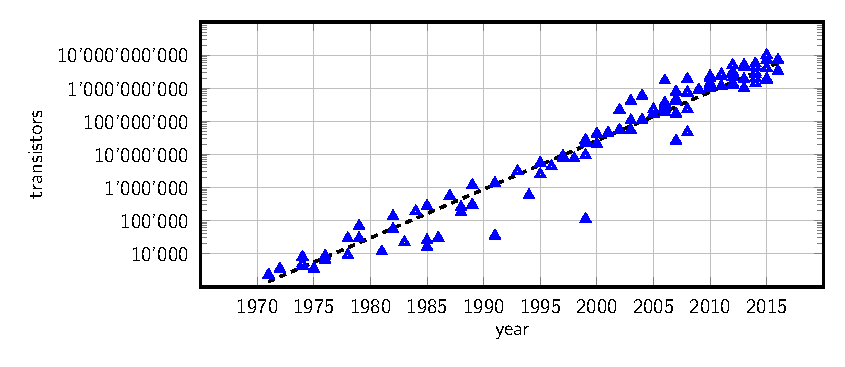
\includegraphics[height=0.5\textheight]{transistors.pdf}

\vfill
\end{frame}

%--
\begin{frame}
\frametitle{The limits of frequency}

\vfill
Processor clock speed growth suddenly slowed around 2004.

\vfill
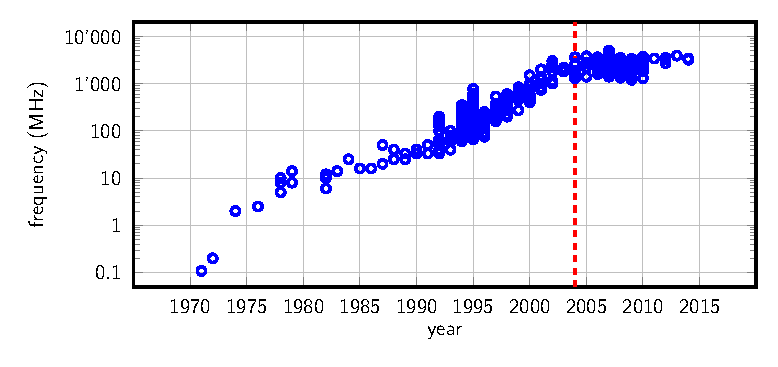
\includegraphics[height=0.45\textwidth]{frequency.pdf}

\vfill
\centering
\textbf{Problem:} $\quad\hbox{power}\ \propto\ \hbox{frequency}^3$

\vfill
\end{frame}


\begin{frame}
\frametitle{The limits of frequency}
\vfill
Single-thread performance growth also slows.

\vfill
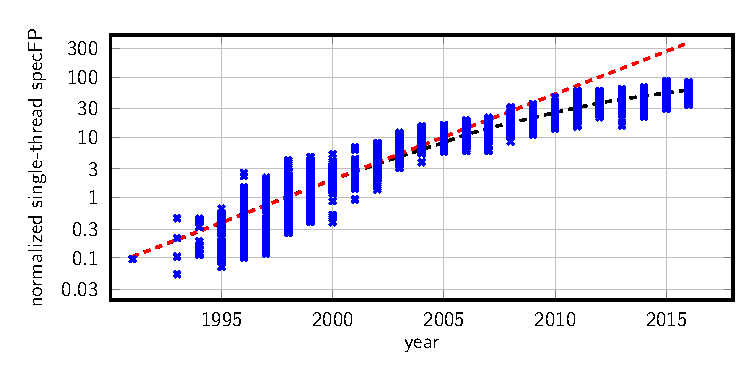
\includegraphics[height=0.5\textwidth]{fp-performance.pdf}

\vfill
\hfill{\scriptsize Analysis thanks to Jeff Preshing, http://preshing.com}
\end{frame}

%--
\begin{frame}
\frametitle{New HPC architectures}

\vfill
New performance gains primarily from:

\vfill
\begin{itemize}
\item Highly parallel architectures (e.g. Intel KNL).
\item Wider vector operations (e.g. AVX512).
\item Specialized accelerator hardware: GPU, FPGA.
\end{itemize}

\vfill
\end{frame}

%--
\begin{frame}
\frametitle{New HPC architectures}

\centering
Prototype Human Brain Project HPC systems at J\"ulich\\

\vfill
\begin{minipage}[t][0.3\textheight][t]{0.4\textwidth}
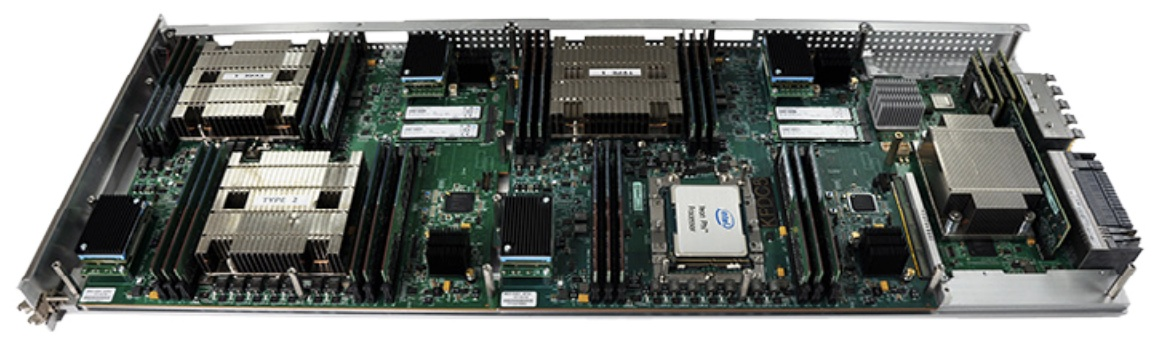
\includegraphics[width=\textwidth]{images/knlnode.jpg}

\vfill
{\small\centering
Julia\\
\em Intel many core KNL blade}
\end{minipage}
\hfill
\begin{minipage}[t][0.4\textheight][t]{0.4\textwidth}
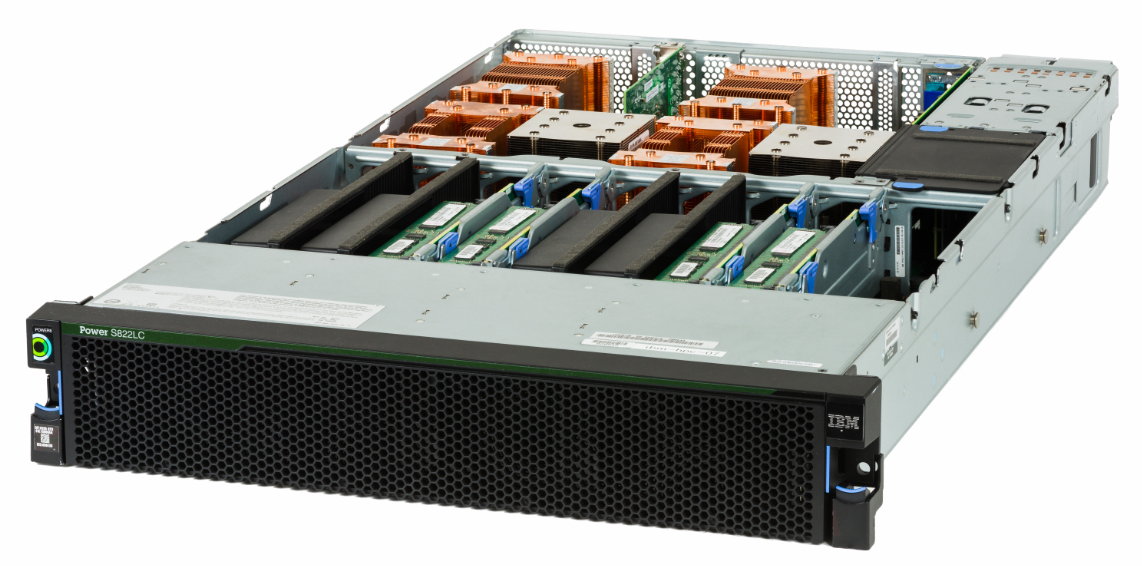
\includegraphics[width=\textwidth]{images/juron.jpg}

\vfill
{\small\centering
Juron\\
\em IBM Power8+GPU `fat' node}
\end{minipage}
\\[2ex]

\vfill
Efficient use demands new approaches.\\
We no longer get good performance improvement `for free'.

\vfill
\end{frame}

%--
\begin{frame}
\frametitle{Why?}
\subheading{Why develop a new simulator?}
\vfill
\begin{itemize}
\item
\textcolor{light-grey}{%
There are problems and models that we can't explore
with current software and systems.}
\item
\textcolor{light-grey}{%
New HPC architectures.
}
\item
Adapting existing simulators to new architectures is \emph{hard}.
\end{itemize}
\vfill
\end{frame}

%--
\begin{frame}
\frametitle{Existing simulators}

\textsc{Neuron} and \textsc{Genesis} have had a very long development.
\textsc{Neuron} in particular is very large with many features.

\vspace{2ex}
Newer simulators such as \textsc{Moose} and Brian still primarily
target the workstation.

\vspace{2ex}
GPU support for these simulators still under development.

\vspace{2ex}
\emph{Adapting existing large applications to highly parallel
and hardware-accelerated architectures is non-trivial.}

\end{frame}

%--
\begin{frame}
\frametitle{Opportunity}
A new development project can:
\vfill
\begin{itemize}
\item target contemporary and future HPC architectures,
\item be co-designed to faciliatate new and difficult use cases.
\end{itemize}

\vfill
\pause
In addition,
\begin{itemize}
\item much easier to adopt modern software development processes from the start.
\end{itemize}
\vfill
\end{frame}

%--
\begin{frame}
\frametitle{\nestmc}
\vspace{2ex}
Two year initial project to design and develop
a multi-compartmental simulator for HPC systems.

\vfill
\begin{center}\bf Goals\end{center}

\vfill
\begin{columns}[t,onlytextwidth]
\column{0.3\textwidth}
\centering Interoperability
\\[2ex]
\small
{\em Simulator as library}
\\
\begin{itemize}
\small
\setlength{\itemsep}{0.2ex}
\item Visualization
\item Multi-physics
\item Multi-scale
\end{itemize}

\column{0.3\textwidth}
\centering Extensibility
\\[2ex]
\small
{\em Modular internal API}
\\
\begin{itemize}
\small
\setlength{\itemsep}{0.2ex}
\item New integration schemes
\item Custom spike communication
\item Specialized cells
\end{itemize}

\column{0.3\textwidth}
\centering Performance
\\[2ex]
\small
{\em HPC targeted}
\begin{itemize}
\small
\setlength{\itemsep}{0.2ex}
\item Highly parallel
\item GPU and vector targets
\item Design for scalability
\end{itemize}

\end{columns}

\vspace{4ex}
\end{frame}

%--
\begin{frame}
\frametitle{Development timeline}

\textbf{Now}\\[1ex]
\hspace{2cm}Prototype development.

\vspace{2em}
\textbf{12/2016}\\[1ex]
\hspace{2cm}Wind-up prototype.\\
\hspace{2cm}Finalize design of initial release.

\vspace{2em}
\textbf{4/2017}\\[1ex]
\hspace{2cm}First public release of simulator.\\
\hspace{2cm}Move to open development model.\\


\end{frame}
%--
\begin{frame}
\frametitle{Prototype}

The prototype development allows us to explore the design space.
\\
\hfill\textit{``Plan one to throw one away'' --- Fred Brookes}

\vfill
Currently implementing features and use cases to refine our design:

\begin{itemize}
\item LFP live visualization $\to$ interoperability features.
\item Gap junctions $\to$ extensibility, internal API design.
\item GPU execution $\to$ performance, modularity.
\end{itemize}

\vfill
\end{frame}

%--
\begin{frame}
\frametitle{Prototype design}
Modular: components can be substituted according to internal API.

\vspace{2ex}
Internal API: `thin' API; type parameterization allows components
to determine low-overhead API data structures.

\vspace{2ex}
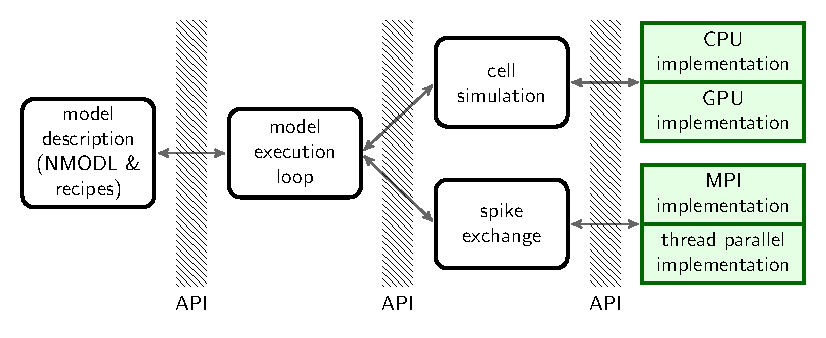
\includegraphics[width=\textwidth]{api.pdf}
\end{frame}

%--
\begin{frame}
\frametitle{Prototype design --- backends}

Cell simulation modules share computational backends for channel
and synapse state evolution.

\vfill
\centering
CPU-hosted finite volume cell simulation\\
\vspace{2ex}
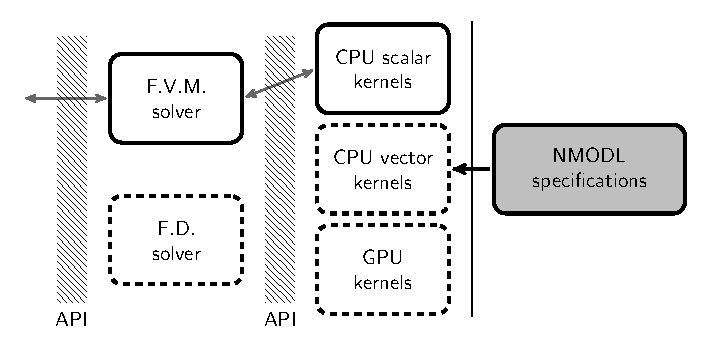
\includegraphics[height=0.5\textheight]{backend-api.pdf}

\vfill
\end{frame}

%--
\begin{frame}
\frametitle{Prototype status}

\subheading{Currently implemented}

\vfill
\begin{itemize}
\item Finite-volume based discretization.
\item Distributed model instantiation.
\item Spike and voltage trace output.
\item x66 multi-core and Intel KNL support.
\item Synapse and ion-channel descriptions in NMODL.
\item Unit and validation testing suite.
\item GPU support (almost!)
\end{itemize}

\vfill
\vspace{4ex}
\end{frame}

%--
\begin{frame}
\frametitle{Prototype benchmarks}
\subheading{Test case}

\vfill
\begin{itemize}
\item 500~ms simulation.
\item Each cell has 350 compartments and 2000 exponential excitatory synapses.
\item H--H mechanism on cell somas, passive dendrites.
\item Random network.
\item Approximately 50~Hz spiking rate.
\end{itemize}

\vfill
Benchmarks run on \emph{Pitz Dora}, a Cray XC-40 system with 36 Broadwell cores per node.

\vfill
\end{frame}

%--
\begin{frame}
\frametitle{Prototype benchmarks --- strong scaling}
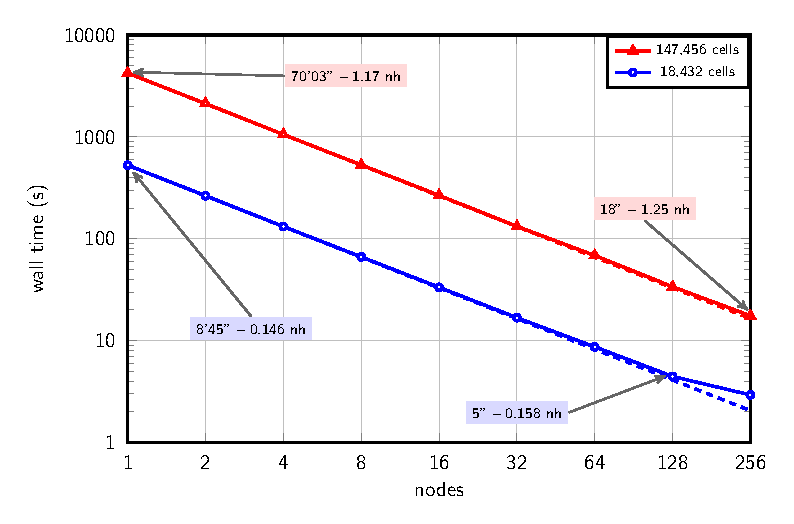
\includegraphics[width=\textwidth]{strong.pdf}

\vfill
\end{frame}

%--
\begin{frame}
\frametitle{Prototype benchmarks --- weak scaling}
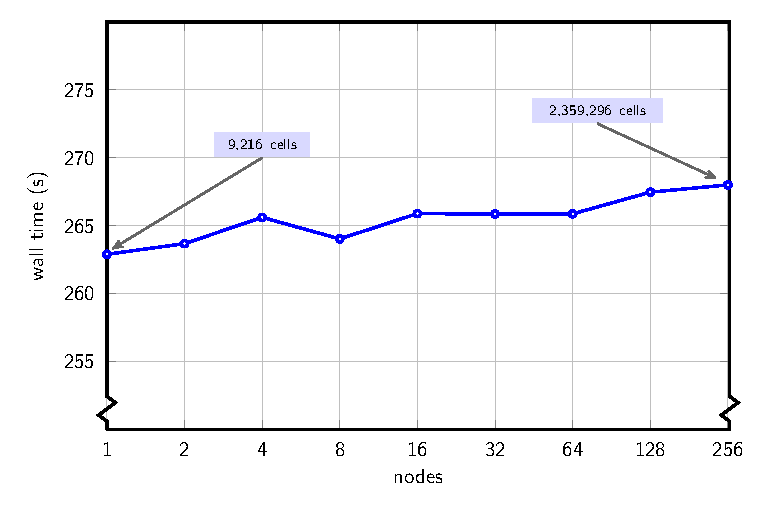
\includegraphics[width=\textwidth]{weak.pdf}

\vfill
\end{frame}

%--
\begin{frame}
\frametitle{Prototype observations}
\subheading{Design}

\vfill
\begin{itemize}
\item Abstractions over communication and threading\\
\hspace{5mm} $\to$ greatly simplified testing and validation.
\item Component architecture\\
\hspace{5mm} $\to$ rapid prototyping,\\
\hspace{5mm} $\to$ use-case driven API changes are limited in scope.
\item Functional model description\\
\hspace{5mm} $\to$ reproducible across different systems,\\
\hspace{5mm} $\to$ distributed instantiation.
\end{itemize}
\vfill
\end{frame}

%--
\begin{frame}
\frametitle{Prototype observations}
\subheading{Development practices}

\vfill
\begin{itemize}
\item Unit and validation testing\\
\hspace{5mm} $\to$ limits exposure to bugs and design errors.
\item Large matrix of compilers and hardware targets\\
\hspace{5mm} $\to$ continuous integration a necessity\\
\item `Agile' iterative refinement of development practices allows us
to adapt our processes to our team distributed across multiple institutions and countries.
\end{itemize}

\vfill
\end{frame}

%--
\begin{frame}
\frametitle{Participate}

\vfill
\begin{center}
Success depends on facilitating use cases!
\end{center}

\vfill
\emph{Do you have a use case which is hard to simulate with current tools?}

\vfill
\emph{Are there computational experiments that you wish to run, but currently cannot?}

\vfill
We want to work closely with researchers and research groups to ensure
that our designs meet real needs in the community. 

\vfill
\end{frame}

%************************************************
\begin{frame}[noframenumbering,plain]
\cscsthankyoucontent{}
\begin{picture}(0,0)
   \put(-18,-70){\bf Contact}
   \put(60,-70){
       \begin{minipage}[t]{10em}
	  \tt
	  \textcolor{cscsgrey}{bcumming@cscs.ch}\\
	  \textcolor{cscsgrey}{a.peyser@fz-juelich.de}\\[2ex]
	  \textcolor{cscsblue}{https://eth-cscs.github.io/nestmc}
       \end{minipage}
   }
\end{picture}
\end{frame}

\end{document}
